\documentclass[tikz,border=4pt]{standalone}
\usepackage{amsmath,amssymb}
\usetikzlibrary{arrows.meta,calc,decorations.pathreplacing}
\definecolor{cA}{HTML}{924800}
\definecolor{cB}{HTML}{2F7FC8}
\definecolor{cC}{HTML}{39994B}
\tikzset{
  pt/.style={circle,fill=black,inner sep=0pt,minimum size=4pt},
  disp/.style={-{Stealth[length=2.6mm,width=2mm]},line width=0.9pt,shorten <=2.5pt,shorten >=2.5pt},
  lab/.style={font=\small,sloped,text=black},
  brc/.style={decorate,decoration={brace,amplitude=5pt,raise=3pt},line width=0.6pt},
}
\begin{document}
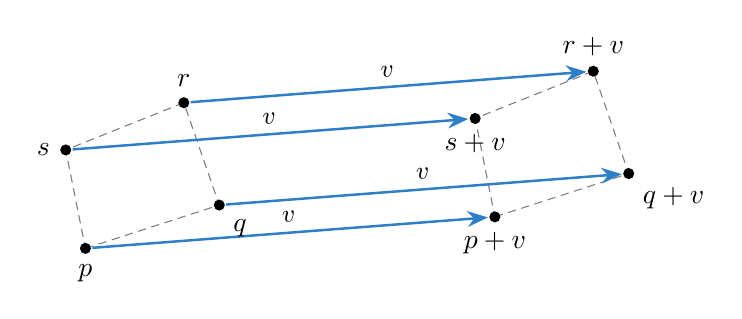
\begin{tikzpicture}
  \coordinate (v) at (5.2,0.4);
  \coordinate (p) at (0,0); \coordinate (q) at (1.7,0.55); \coordinate (r) at (1.25,1.85); \coordinate (s) at (-0.25,1.25);
  \draw[densely dashed,gray] (p)--(q)--(r)--(s)--cycle;
  \draw[densely dashed,gray] ($(p)+(v)$)--($(q)+(v)$)--($(r)+(v)$)--($(s)+(v)$)--cycle;
  \foreach \x in {p,q,r,s} \draw[disp,cB] (\x) -- node[lab,above,pos=0.5]{$v$} ($(\x)+(v)$);
  \foreach \x/\pos/\posv in {p/below/below,q/below right/below right,r/above/above,s/left/below}{
    \node[pt,label=\pos:$\x$] at (\x) {};
    \node[pt,label=\posv:$\x+v$] at ($(\x)+(v)$) {};
  }
\end{tikzpicture}
\end{document}
